\section{Sweep}
\begin{frame}
	\begin{center}
		\textbf{Sweep}
	\end{center}
\end{frame}

\subsection{Line Segment Intersection}
\begin{frame}
	\frametitle{{Line Segment Intersection}}
	\begin{block}{Das Problem}
	\begin{itemize}
		\pause
		\item{Eingabe:}
		\pause
		\begin{itemize}
			\item{n Liniensegmente}
		\end{itemize}
		\pause
		\item{Ausgabe:}
		\pause
		\begin{itemize}
			\item{Anzahl der Schnittpunkte}
		\end{itemize}
	\end{itemize}
	\end{block}
\end{frame}
\begin{frame}
	\frametitle{{Line Segment Intersection}}
	\begin{itemize}
		\item \textbf{Anwendungsbeispiel}
		\item Schnitt von Layern bei Kartographie-Software
	\end{itemize}
	\begin{figure}
  		\begin{center}
   			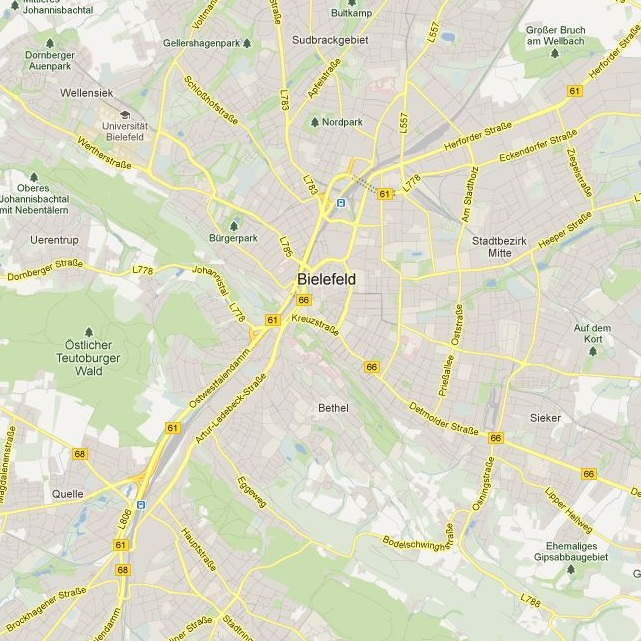
\includegraphics[scale=0.30]{bilder/map.jpg}
 		\end{center}
	\end{figure}
\end{frame}
\begin{frame}
	\frametitle{{Line Segment Intersection}}
	\begin{itemize}
		\item \textbf{Naiv}
		\begin{itemize}
			\pause
			\item{Vergleiche jedes Segment mit jedem anderen}
			\pause
			\item{Resultierende Laufzeit: $\mathcal O(n^2)$}
		\end{itemize}
	\end{itemize}
\end{frame}
\begin{frame}
	\frametitle{{Line Segment Intersection}}
	\begin{itemize}
		\item \textbf{Weitere \"Uberlegungen}
		\pause
		\item{Nur nahe Segmente k\"onnen sich schneiden}
		\pause
		\item{Betrachten der Situation an der Stelle a}
	\end{itemize}
\end{frame}
\begin{frame}
	\frametitle{{Line Segment Intersection}}
	\begin{itemize}
		\item \textbf{Sweep Line Algorithmus, erster Ansatz}
		\pause
	\end{itemize}
	\begin{block}{Ben\"otigte Daten}
		\begin{itemize}
			\item Zustand der Sweep Line S
			\begin{itemize}
				\item Segmente, welche die Sweep Line schneiden
			\end{itemize}
			\pause
			\item Event Queue Q
			\begin{itemize}
				\item Endpunkte der Segmente, aufsteigend geordnet nach ihrer x-Koordinate
			\end{itemize}
		\end{itemize}
	\end{block}
	\begin{itemize}
		\pause
		\item Beginnt ein Segment
		\begin{itemize}
			\pause		
			\item F\"uge das Segment dem Zustand hinzu
			\pause
			\item \"Uberpr\"ufe, ob es Segmente in S schneidet
		\end{itemize}
		\pause
		\item Endet ein Segment
		\begin{itemize}
			\pause
			\item Entferne das Segment aus dem Zustand
		\end{itemize}
		\pause
		\item Das geht noch besser!
	\end{itemize}
\end{frame}
\begin{frame}
	\frametitle{{Line Segment Intersection}}
	\begin{itemize}
		\item \textbf{Sweep Line Algorithmus}
		\pause
		\item Verlgeiche nur direkt benachbarte Segmente
		\pause
		\item Neuer Eventpunkt:
		\begin{itemize}
			\pause
			\item Beim Schnitt zweier Segmente
		\end{itemize}
	\end{itemize}
	\pause
	\begin{block}{Ben\"otigte Daten}
		\begin{itemize}
			\item Zustand der Sweep Line S
			\begin{itemize}
				\item Segmente, welche die Sweep Line schneiden
				\pause
				\item F\"ur jedes Segment die Nachbarn
			\end{itemize}
			\pause
			\item Event Queue Q
			\begin{itemize}
				\item Endpunkte der Segmente
				\pause
				\item Schnittpunkte zwischen Segmenten
			\end{itemize}
		\end{itemize}
	\end{block}
	\pause
	\begin{itemize}
		\item Bentley Ottmann Algorithmus
		\begin{itemize}
			\item Laufzeit $\mathcal O((n+k)\cdot log(n))$
		\end{itemize}
	\end{itemize}
\end{frame}

\subsection{Allgemeine Eigenschaften}
\begin{frame}
	\frametitle{{Allgemeine Eigenschaften von Sweep Algorithmen}}
	\begin{itemize}
		\item Anwendbar auf Probleme beliebig hoher Dimension
		\begin{itemize}
			\pause
			\item{Im 2-Dimensionalen Raum}
			\begin{itemize}
				\item{Gerade, die \"uber sich über die Ebene bewegt}
			\end{itemize}
			\pause
			\item{Im 3-Dimensionalen Raum}
			\begin{itemize}
				\item{Ebene, die sich durch den Raum bewegt}
			\end{itemize}
		\end{itemize}
	\end{itemize}
\end{frame}

\subsection{Weitere Algorithmen}
\begin{frame}
	\frametitle{{Weitere Sweep Algorithmen}}
	\begin{itemize}
		\pause
		\item Fortune's algorithm
		\begin{itemize}
			\item Sweep Line Algorithmus zur Erstellung eines Voronoi-Diagramms
			\pause			
			\item M\"ogliches Anwendungsgebiet: Robotik, Hindernissen fern bleiben
		\end{itemize}
		\pause
		\item Boolsche Operationen auf Polygone
		\begin{itemize}
			\item M\"ogliche Anwendungsgebiete: Computergraphik oder CAD-Systeme
		\end{itemize}
		\pause
		\item Closest Pair
		\pause
		\item Viele mehr!
	\end{itemize}
\end{frame}
